\section{Layoutplanung}

\textbf{Aufgabe:} 
\begin{itemize}
	\item Räumlichen Anordnung von \textbf{Anordnungsobjekten (AO)} in einer Einrichtung zur Güterproduktion oder Serviceerbringung
	\item Anordnung erfolgt auf Basis der Einrichtungsprämissen und so, dass eine gegebene Zielgröße optimiert wird
	\item \textbf{Beispiel}: Anordnung der Krankenhausräume zur Minimierung der Patientenwege
\end{itemize} 
\pagebreak
\textbf{Relevanz von Layoutplanung:}
\begin{itemize}
	\item Layoutplanung beeinflusst die Produktionskapazität, Produktionskosten, Prozessorganisation und Arbeitssicherheit eines Unternehmens
	\item Umplatzierung ist mit vielen Kosten und Betriebsstopp verbunden 
	
	$\rightarrow$ Beeinflusst die langfristige Wettbewerbsfähigkeit eines Unternehmens
\end{itemize}
\bigskip
\textbf{Anlässe für Layoutplanung:}
\begin{itemize}
	\item \textbf{Neugestaltung}: Erstmalige Gestaltung eines Layouts
	\item \textbf{Erweiterung}: Zusätzliches AO in existierendes Layout integrieren
	\item \textbf{Umstellung}: Veränderung des bestehenden Layouts $\rightarrow$ \textbf{Demontagekosten}
\end{itemize}
\bigskip
\textbf{Anwendungsgebiete von Layoutplanung}:
\begin{itemize}
	\item \textbf{Service-System-Layouts}: Direkter Kundenkontakt $\rightarrow$ Ziel: Wohlbefinden des Kunden (Bsp. Krankenhaus, Verwaltungsstellen, Shops)
	\item \textbf{Produktions-Layouts}: Transportaufwand vieler Güter innerhalb der Produktionsanlage $\rightarrow$ Ziel: Geringe Transportkosten/-zeiten, Arbeitssicherheit
	\item \textbf{Lagerhaus-Layouts}: Lagerung von Erzeugnissen und Materialien $\rightarrow$ Ziel: Minimierung Lagerkosten sowie Einlagerungs- und Entnahmezeiten
	\item \textbf{Nicht-traditionelle Layout-Probleme}: Tastaturlayouts
\end{itemize}
\bigskip
\textbf{Layouttypen:}
\begin{center}
	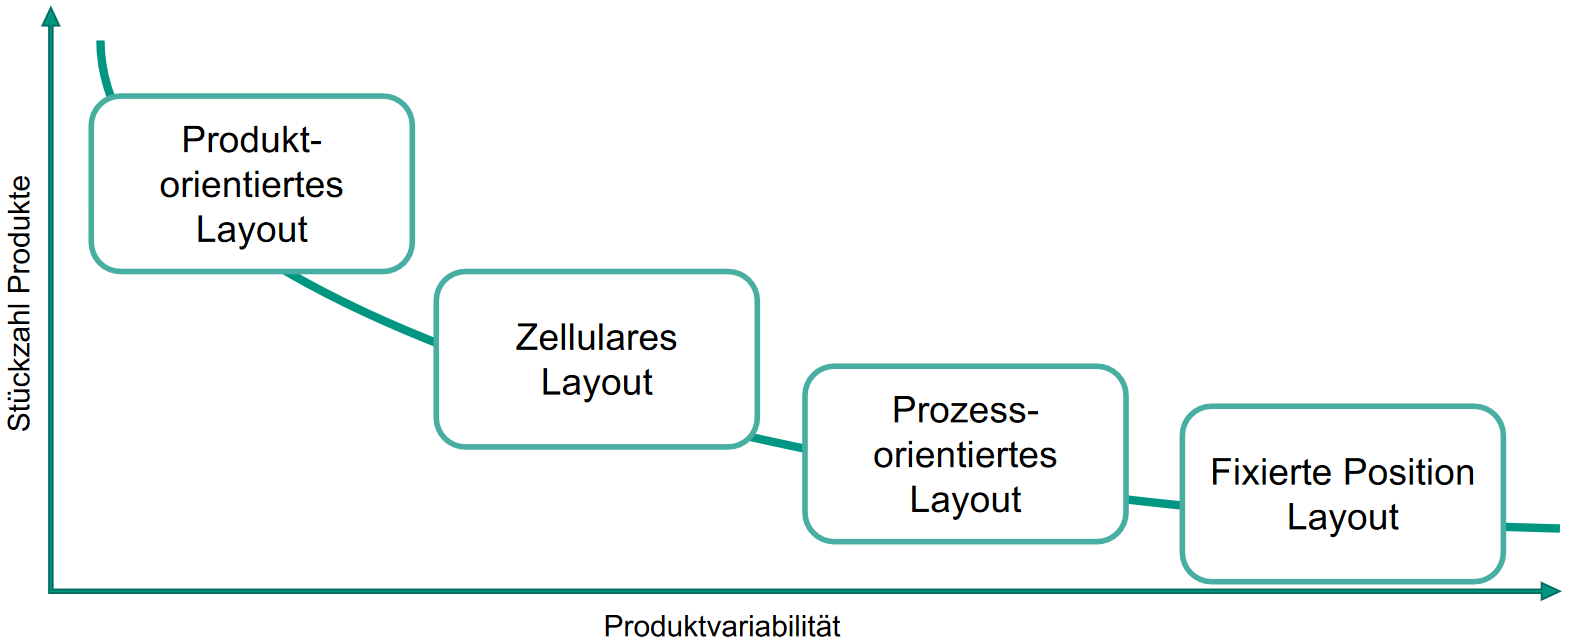
\includegraphics[width=0.7\textwidth]{images/layout-types.png}
\end{center}
\begin{itemize}
	\item \textbf{Produktorientiertes Layout}:
	\begin{itemize}
		\item AOs sind entsprechend der Fertigungssequenz von Produkten angeordnet, z.B. Fließbandsysteme
		\item \textbf{Vorteil}: Hohes Produktionsvolumen, geringe Stückkosten
		\item \textbf{Nachteil}: Geringe Produktvariabilität, geringe Flexibilität für neue Produkte $\rightarrow$ Nachfrage muss stabil bleiben, hohe Kapitalkosten
	\end{itemize}
	\item \textbf{Zellulares Layout}:
	\begin{itemize}
		\item AOs in Subsysteme zusammengefasst, in denen die Produktion stattfindet
		\item \textbf{Vorteil}: Geringere Raumbelegung, Geringere Arbeitskosten, Geringerer Work-in-Process Inventarbedarf
		\item \textbf{Problem}: Intra-Zell-Maschinen-Layout
	\end{itemize}
	\item \textbf{Prozessorientiertes Layout}:
	\begin{itemize}
		\item AOs werden einzeln platziert, Produkte werden zwischen AOs transportiert
		und haben individuelle AO-Reihenfolge $\rightarrow$ \textbf{Ziel}: Minimierung der Transportaufwendungen
		\item \textbf{Vorteil}: Hohe Produktvariabilität, einfaches Integrieren neuer Produkte, geringe Kapitalkosten
		\item \textbf{Nachteile}: Hohe Stückkosten, geringes Produktionsvolumen
		\item \textbf{Typisches Problem}: \textbf{Quadratisches Zuordnungsproblem}
	\end{itemize}
	\item \textbf{Fixierte Position Layout}: 
	\begin{itemize}
		\item Produkt ist fest platziert, AOs bewegen sich um das Produkt
		\item \textbf{Anwendung}: Große, schwer transportierbare Einzelprodukte, z.B. Werften, Flugzeugfabrik
	\end{itemize}
\end{itemize}

\subsection{Quadratisches Zuordnungsproblem (QZP)}
\begin{center}
	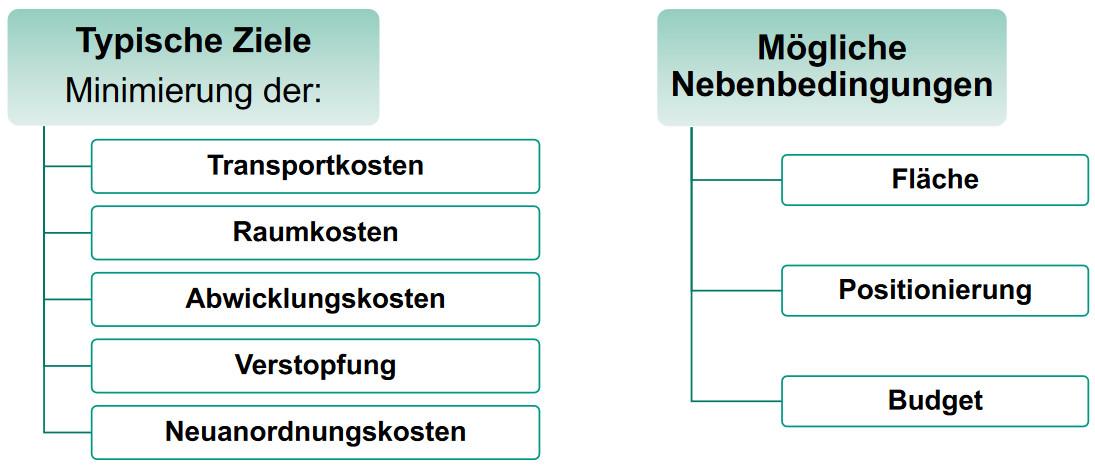
\includegraphics[width=0.6\textwidth]{images/goals.png}
\end{center}

\textbf{Annahmen des klassischen QZP:}
\begin{itemize}
	\item $p$ gleichgroße AOs müssen auf diese $p$ gleichgroße Positionen platziert werden
	\item Für alle $k,l=1,\ldots,p$ ist $d_{kl}$ die Distanz von $k$ nach $l$, es gilt $d_{kk}=0$ $\rightarrow$ Distanzmatrix $(D)_{kl}$
	\item Zwischen den AOs findet Warenaustausch mit Häufigkeit $h_{ij}$ von $i$ nach $j$ statt $\rightarrow$ Häufigkeitsmatrix $(H)_{ij}$
	\item Ziel: Gesamttransportkosten (abh. von Distanzen und Häufigkeiten) minimieren
\end{itemize}
\bigskip
\textbf{Mathematische Formulierung als ganzzahliges Programm:} 
\begin{itemize}
	\item \textbf{Entscheidungsvariable} $x_{ik}=
	\begin{cases}
		1\;, & \text{wenn AO } i \text{ an Position } k \text{ zugeordnet ist}\\
		0\;, & \text{sonst}
	\end{cases}$ 
	\item \textbf{Zielfunktion}: $\sum\limits_{i=1}^{p}\sum\limits_{\substack{j=1 \\ j\neq i}}^{p}\sum\limits_{k=1}^{p}\sum\limits_{\substack{l=1 \\ k\neq l}}^{p} h_{ij}d_{kl}x_{ik}x_{jl}\rightarrow\min$
	\item \textbf{Nebenbedingungen}: 
	\begin{itemize}
		\item Jedes AO ist exakt einer Position zugeordnet: $\sum\limits_{k=1}^{p}x_{ik}=1 \;\; \forall i=1,\ldots,p$
		\item Jede Position ist zu genau einem AO zugeordnet: $\sum\limits_{i=1}^{p}x_{ik}=1 \;\; \forall k=1,\ldots,p$
		\item Binarität der Entscheidungsvariable: $x_{ik}\in\{0,1\}\;\; \forall i,k=1,\ldots,p$
	\end{itemize}
	\item Bei zusätzlicher Distanzsymmetrie ($d_{kl}=d_{lk}$) kann Zielfunktion gekürzt werden: $\sum\limits_{i=1}^{p-1}\sum\limits_{j=i+1}^{p}\sum\limits_{k=1}^{p}\sum\limits_{\substack{l=1 \\ l\neq k}}^{p} (h_{ij}+h_{ji})d_{kl}x_{ik}x_{jl}\rightarrow\min$
\end{itemize}
\textit{Beispiele siehe Tut 4 und Logistik VL 4, F19-23}

\subsection{Zweiertauschverfahren}
\textbf{Vorgehen}: 
\begin{enumerate}
	\item Ausgang: Layout mit Startlösung gegeben
	\item Berechne für alle Paare $(k,l)$ von Standorten den Zielfunktionswert, wenn man die AOs auf den Positionen tauscht
	\item Wenn kein niedrigere Zielfunktionswert gefunden: STOP, sonst führe 2. mit der Zuordnung mit dem neuen geringsten Zielfunktionswert aus
\end{enumerate}

\textit{Beispiele siehe Logistik VL 4, F32-35}